\chapter{Introduction}

Rare Earth Elements (REEs) play a critical role in modern-day life.
They are used in nearly every device that uses electrical power to operate.
A few examples where REEs are essential are: lasers, computer monitors, electric motors, electric generators, high-power magnets, liquid crystal displays (LCDs), solar panels and many more~\cite{usageofrees}.

\begin{figure}[H]
    \centering
    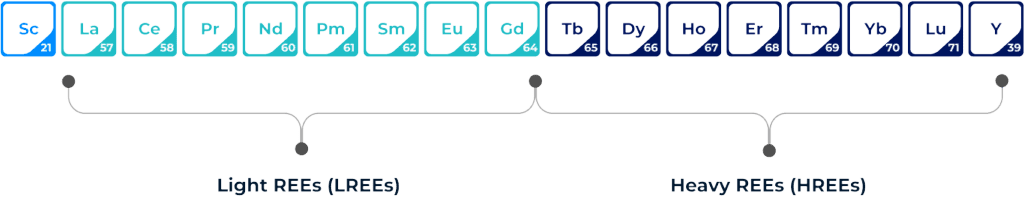
\includegraphics[width=0.9\textwidth]{./media/images/rees_periodic_table}
    \caption{List of all rare earth elements. Those 16 elements can be further categorized into the light rare earth elements (LREEs) and the heavy rare earth elements (HREEs). Picture from lynasrareeaths.com.}
    \label{fig:list_rees}
\end{figure}


\section{Problem Setting\authorA{}}

Given the importance of REEs in the modern world, it is evident that the demand for them is increasing quickly.
In the coming years, as the use of electronic devices increases, many of them will become electronic waste.
It is vital for the world's future supply of rare earth elements to recycle them from this waste.

Currently used recycling methods for REEs are mostly damaging to the environment and very costly~\cite{recyclingcurrent}.
Therefore, only around one percent of the global REE usage is from recycled sources~\cite{currentrecyclingnumbers}.
The rest comes from mining, which brings its own challenges.
Rare earth ores (REOs) often contain radioactive elements which adds more complexity to the processing of the ores.
Also, the extraction of REEs is done by using a process called flotation which produces large amounts of waste water.
This waste water is highly problematic, as it often contains radioactive minerals, acids and toxic agents~\cite{reeenvimpact}.

There are already thousands of tonnes of electronic waste that contain significant amounts of REEs. Recycling them would reduce the need of mining new REOs and therefore reduce the environmental impact of new electronic devices.
Sadly, there is no easy and environmentally friendly process to recycle REEs on an industrial scale.


\section{Inventions OR Solutions OR Contributions}

Lorem ipsum dolor sit amet, consectetur adipiscing elit. Aenean viverra eget sapien in fringilla. Proin ac neque non lectus vehicula laoreet in cursus enim. Donec et erat ut erat commodo viverra vitae sed risus. Etiam tortor justo, placerat in turpis sit amet, egestas tristique libero. Phasellus metus arcu, viverra at interdum ac, convallis non urna. Sed nunc libero, elementum quis ultricies at, vestibulum in arcu. Nam ultrices felis ut sagittis hendrerit. Vivamus massa sapien, interdum nec dui ac, consectetur venenatis dolor. Integer enim felis, finibus at efficitur eget, viverra vitae purus. Curabitur at libero pretium, vestibulum lacus at, eleifend nisl.

Nullam ut magna quis ante gravida aliquet. Integer ultricies libero vitae quam mollis, non tincidunt justo posuere. Mauris ultricies varius orci non tempus. Sed at ex maximus, tempor libero id, convallis ligula. Donec posuere massa sit amet porttitor vehicula. Donec porttitor luctus dui sed blandit. Ut egestas, enim id egestas auctor, est ligula accumsan diam, nec lacinia massa elit vitae purus.

Ut consectetur ipsum id nisl sodales varius. Pellentesque habitant morbi tristique senectus et netus et malesuada fames ac turpis egestas. Aliquam venenatis varius maximus. Aenean aliquet mi a magna tempor, et sagittis ligula tincidunt. Maecenas ornare non leo et dignissim. Nunc ac feugiat magna. Nulla at sollicitudin massa, nec sollicitudin libero. Nunc posuere dolor mauris, non congue neque lobortis eget. Vestibulum ex leo, ullamcorper quis malesuada in, maximus quis nisl. Morbi neque diam, dignissim non suscipit ac, molestie at sem. In hac habitasse platea dictumst. Curabitur dictum eros non ipsum luctus, a malesuada sapien iaculis. Nam mauris nisi, sodales et consectetur quis, varius eu lacus.


\section{Structure of this Thesis}

Lorem ipsum dolor sit amet, consectetur adipiscing elit. Aenean viverra eget sapien in fringilla. Proin ac neque non lectus vehicula laoreet in cursus enim. Donec et erat ut erat commodo viverra vitae sed risus. Etiam tortor justo, placerat in turpis sit amet, egestas tristique libero. Phasellus metus arcu, viverra at interdum ac, convallis non urna. Sed nunc libero, elementum quis ultricies at, vestibulum in arcu. Nam ultrices felis ut sagittis hendrerit. Vivamus massa sapien, interdum nec dui ac, consectetur venenatis dolor. Integer enim felis, finibus at efficitur eget, viverra vitae purus. Curabitur at libero pretium, vestibulum lacus at, eleifend nisl.

Nullam ut magna quis ante gravida aliquet. Integer ultricies libero vitae quam mollis, non tincidunt justo posuere. Mauris ultricies varius orci non tempus. Sed at ex maximus, tempor libero id, convallis ligula. Donec posuere massa sit amet porttitor vehicula. Donec porttitor luctus dui sed blandit. Ut egestas, enim id egestas auctor, est ligula accumsan diam, nec lacinia massa elit vitae purus.

Ut consectetur ipsum id nisl sodales varius. Pellentesque habitant morbi tristique senectus et netus et malesuada fames ac turpis egestas. Aliquam venenatis varius maximus. Aenean aliquet mi a magna tempor, et sagittis ligula tincidunt. Maecenas ornare non leo et dignissim. Nunc ac feugiat magna. Nulla at sollicitudin massa, nec sollicitudin libero. Nunc posuere dolor mauris, non congue neque lobortis eget. Vestibulum ex leo, ullamcorper quis malesuada in, maximus quis nisl. Morbi neque diam, dignissim non suscipit ac, molestie at sem. In hac habitasse platea dictumst. Curabitur dictum eros non ipsum luctus, a malesuada sapien iaculis. Nam mauris nisi, sodales et consectetur quis, varius eu lacus.
